Los siguientes son los diferentes diagramas que describen el comportamiento del sistema.

% Diagrama de contexto
\subsection{Diagrama de contexto}
A continuaci'on se diagraman los principales fen'omenos encontrados fuera y para con el sistema.
\imagen{DC_DiagramaDeContexto.png}{Diagrama de contexto}{0.6}
\clearpage


% Modelo de objetivos
\subsection{Modelo de objetivos}
\begin{figure}[p!hbt]
		\centering
		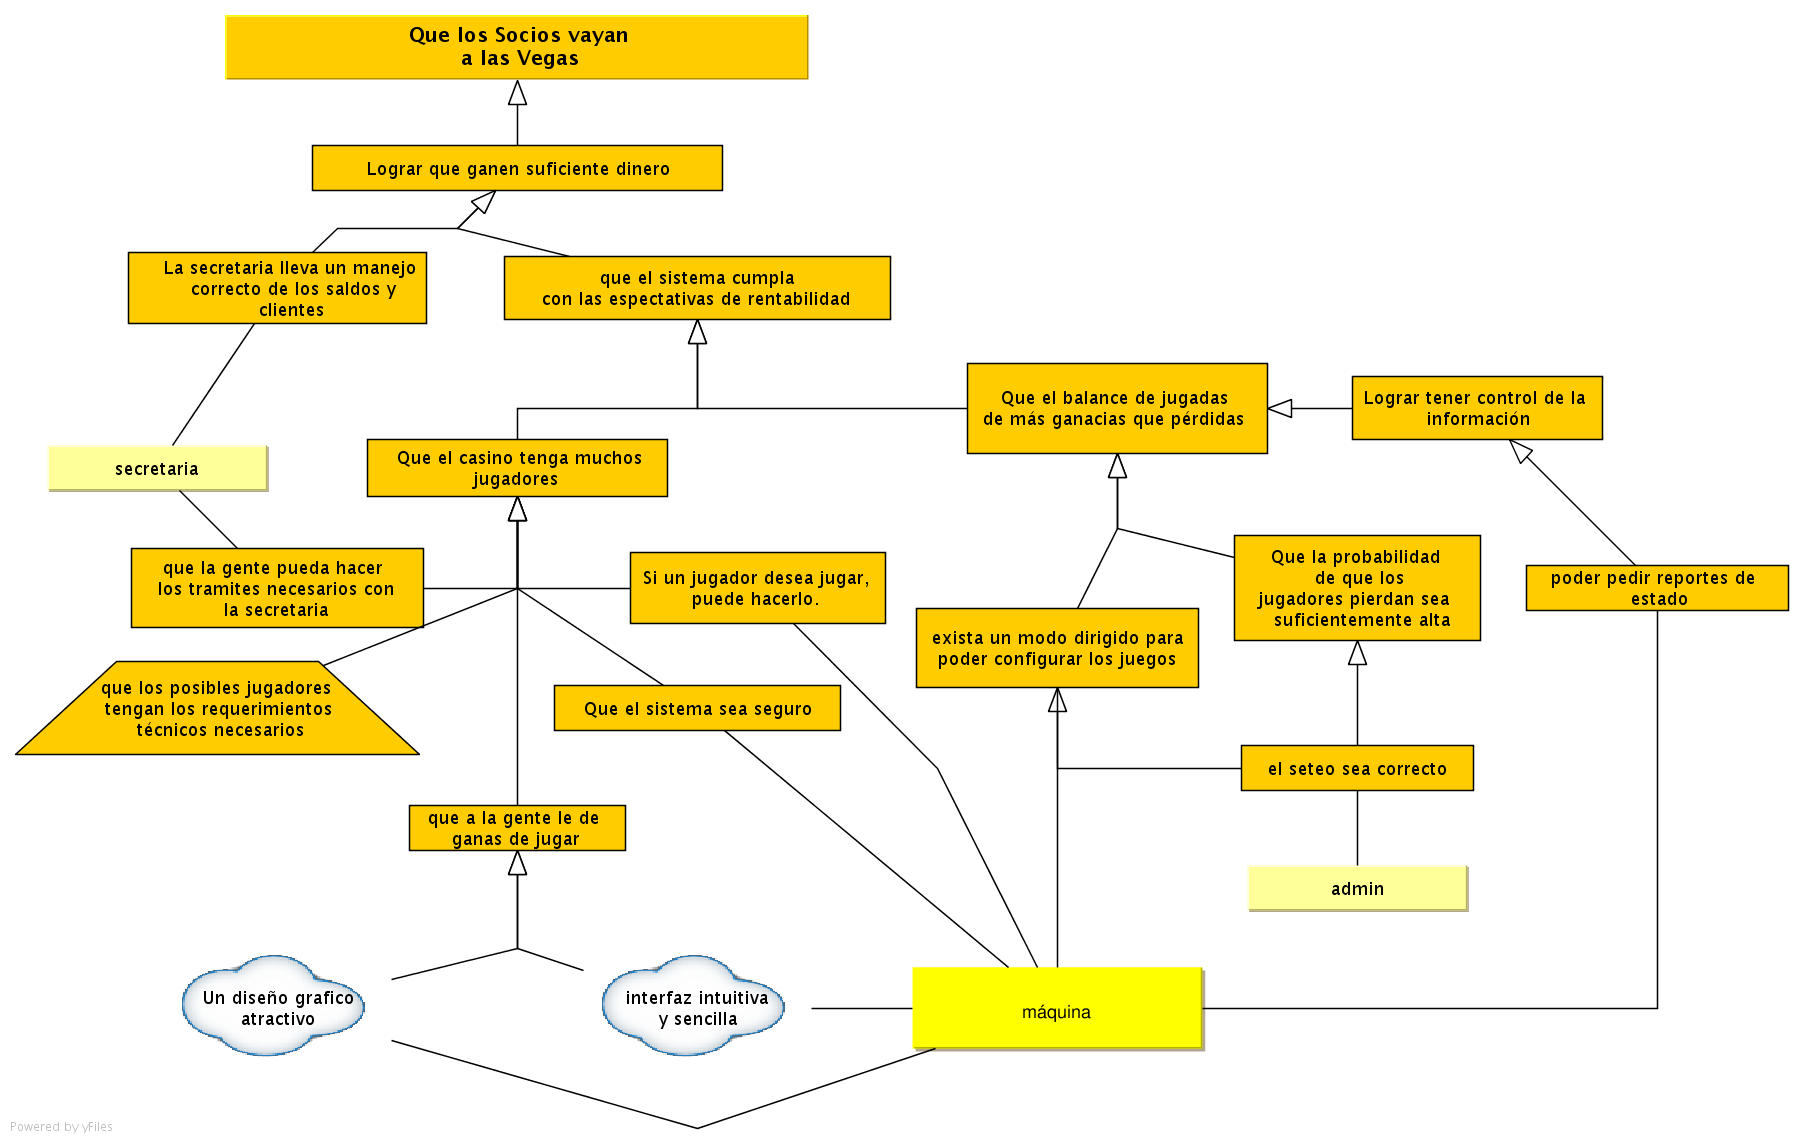
\includegraphics[angle=90, width=0.6\textwidth]{../img/DO.png}
		\caption{Diagrama de Objetivos }
		\label{fig:Objetivos}
	\end{figure}

\clearpage


% Requerimientos
\subsection{Requerimientos}
A continuaci'on se detallan los requerimientos del sistema a construir. Se ha identificado cada requerimiento con un c'odigo 'unico que permite referenciar a dichos requerimientos desde el resto del documento.

\subsubsection{Requerimientos funcionales}


% requerimientos esenciales
\subsubsubsection{Esenciales}

\begin{itemize}

\item \reqEsencial{req:abrir_y_cerrar_casino} \negrita{El sistema permite abrir y cerrar el casino}

    \begin{itemize}
        \item El casino podr'a ser abierto cuando se lo desee por un administrador del sistema. 
        \item El casino podr'a ser cerrado cuando se lo desee por un administrador del sistema, con la condici'on de que no existan jugadores dentro al momento de hacerlo.
    \end{itemize}

\item \reqEsencial{req:carga_clientes} \negrita{El sistema permite la carga de los clientes con sus respectivos saldos}

    Los administradores podr'an ingresar al sistema la lista de usuarios y sus saldos (permitiendo especificar qui'enes son vip).

\item \reqEsencial{req:existe_juego_tragamoneda} \negrita{El sistema cuenta con juegos de tipo Tragamonedas conforme al reglamento proporcionado por los SOCIOS}

    El sistema proveer'a un juego de tipo Tragamonedas con las caracter'isticas del juego real y conforme a las reglas presentadas por los SOCIOS.

\item \reqEsencial{req:existe_juego_craps}\negrita{El sistema cuenta con juegos de tipo Craps conforme al reglamento proporcionado por los SOCIOS}

    El sistema proveer'a un juego de tipo Craps con las caracter'isticas del juego real y conforme a las reglas presentadas por los SOCIOS.

\item \reqEsencial{req:ingreso_y_salida_al_casino}\negrita{El sistema permite a los jugadores ingresar y salir del casino}

    Los jugadores deben poder ingresar al casino utilizando para ello los datos de su cuenta y salir del mismo cuando as'i lo deseen.
 
\item \reqEsencial{req:creacion_ingreso_y_salida_de_mesa}\negrita{El sistema permite a los jugadores crear, ingresar y abandonar mesas de juego}

    \begin{itemize}
        \item Los jugadores que no est'en en una mesa de juego deben poder crear una nueva mesa de juego del tipo que elijan.
        \item Los jugadores que no est'en en una mesa de juego deben poder ingresar a una mesa existente cuando lo deseen, para lo cual el sistema mantendr'a actualizada la informaci'on sobre las mesas existentes.
        \item Los jugadores que est'en en una mesa de juego deben poder salir de la misma.
    \end{itemize}

\item \reqEsencial{req:auto_cerrar_mesas}\negrita{El sistema se encargar'a de cerrar autom'aticamente las mesas que no tengan jugadores} 

    Cuando una mesa de juego haya sido abandonada por el 'ultimo jugador que la utilizaba, la misma ser'a cerrada por el sistema de forma autom'atica.

\item \reqEsencial{req:apuesta_con_fichas}\negrita{El sistema permite configurar el conjunto de valores de fichas que estar'an disponibles a los jugadores para que interact'uen con el casino} 

    Los jugadores solamente podr'an utilizar los valores de fichas configurados para realizar apuestas y al momento de configurar el valor de ficha de una nueva mesa de tragamonedas.

\item \reqEsencial{req:apuesta_a_juegos}\negrita{El sistema permite a los jugadores apostar a los juegos} 

    \begin{itemize}
        \item Los jugadores que se encuentren en una mesa de juego y posean el saldo suficiente deben poder apostar.
        \item Los jugadores vip que se encuentren en una mesa de juego deben poder apostar siempre, incluso si su saldo es insuficiente para realizar una apuesta (los jugadores vip pueden tener saldo negativo).
    \end{itemize}    

\item \reqEsencial{req:saldos_actualizados} \negrita{El sistema actualizar'a el saldo del casino, jugadores y pozos especiales cuando se realicen apuestas y resuelvan jugadas} 

    \begin{itemize}
        \item El sistema se encargar'a de mantener actualizado el saldo del ``pozo feliz'' cuando se realicen jugadas ``feliz'' y ``todos ponen''.
        \item El sistema se encargar'a de mantener actualizado el saldo del ``pozo progresivo'' cuando se realicen jugadas en m'aquinas tragamonedas.
        \item El sistema se encargar'a de mantener actualizados los saldos de los jugadores y del casino.
    \end{itemize}

\end{itemize}


% requerimientos importantes
\subsubsubsection{Importantes}

\begin{itemize}

\item \reqImportante{req:existe_modo_dirigido}\negrita{El sistema permite a un administrador entrar y salir del ``modo dirigido''} 

    Un administrador de sistema puede activar y desactivar el ``modo dirigido'', lo que le permite controlar el azar y asegurar las ganancias del casino.

\item \reqImportante{req:controlar_juegos}\negrita{El sistema permite a un administrador controlar los juegos en ``modo dirigido''}

    \begin{itemize}
        \item Un administrador del sistema en ``modo dirigido'' puede controlar los resultados de los juegos.
        \item Un administrador del sistema en ``modo dirigido'' puede controlar el tipo de jugada (``normal'', ``feliz'' 'o ``todos ponen'') de los juegos.
    \end{itemize}

\item \reqImportante{req:conf_juegos_jugadas_y_pozos}\negrita{El sistema permite la configuraci'on de los juegos, jugadas especiales y pozos especiales al inicio de una jornada}

    Al dar inicio a una jornada el casino permitir'a a un administrador especificar las siguientes configuraciones:
    \begin{itemize}
        \item La probabilidad de ocurrencia de los distintos tipos de figuras de los juegos tragamonedas.
        \item El valor m'inimo posible para el pozo com'un progresivo de los juegos de m'aquinas tragamonedas.
        \item El valor m'inimo de jugadas consecutivas con apuesta m'axima que debe realizar un jugador para tener oportunidad de ganar el ``premio gordo progresivo''.
        \item La probabilidad de ocurrencia de las jugadas especiales (``feliz'' y ``todos ponen'').
    \end{itemize}

\item \reqImportante{req:reportes} \negrita{El sistema llevar'a registro detallado de apuestas y jugadas y permitir'a generar reportes con informaci'on del estado del casino y sus jugadores}
 
    El casino registrar'a la informaci'on necesaria para generar los tipos de reportes solicitados.
    Un administrador de sistema puede pedir 3 tipos de reportes sobre el estado del casino y sus jugadores para mantener control de la rentabilidad y ajustar correctamente los juegos y pozos. A saber:
    \begin{itemize}
        \item {\bf Ranking de jugadores:} Los jugadores que m'as dinero ganaron en el d'ia, desde que abri'o el casino. De manera an'aloga se podr'a consultar los jugadores que m'as dinero perdieron en el d'ia.
        
        \item {\bf Estado actual:} Informe del estado del casino y los clientes, mostrando los saldos de cada uno.
        
        \item {\bf Detalle movimientos por jugador:} Detalle de todos los movimientos (apuestas, premios ganados, monto ganado) desde que ingresaron al casino, de manera que podr'a verse la tendencia de cada uno de los jugadores.
    \end{itemize}

\item \reqImportante{req:acceso_multiple}\negrita{El sistema permite acceder al casino a m'as de un jugador a la vez desde la misma terminal} 

    Dos o m'as jugadores deben poder acceder al casino desde una misma terminal.

\item \reqImportante{req:agregar_juegos}\negrita{El sistema permite ser extendido mediante la incorporaci'on de nuevos juegos} 

    Cuando los SOCIOS lo deseen, podr'an agregar nuevos juegos al sistema, ampliando las opciones para sus clientes.

\end{itemize}


% requerimientos deseables
\subsubsubsection{Deseables}

\begin{itemize}

\item \reqDeseable{req:chat} \negrita{El sistema permite la comunicaci'on v'ia chat entre jugadores de una misma mesa}

    Los jugadores podr'an expresar entre s'i su felicidad por estar jugando.

\item \reqDeseable{req:inv_ingreso_egreso_al_casino} \negrita{El sistema permite a los invitados ingresar y salir del casino}

    Los invitados deben poder entrar y salir del casino sin necesidad de poseer una cuenta de usuario.

\item \reqDeseable{req:inv_mirar_y_salir_mesas}\negrita{El sistema permite a los invitados mirar una mesa de juego existente}

    \begin{itemize}
        \item Los invitados que no est'en mirando una mesa de juego deben poder ingresar a una mesa existente cuando lo deseen.
        \item Los invitados que est'en mirando una mesa de juego deben poder abandonar la misma.
    \end{itemize}

\end{itemize}


\subsubsection{Requerimientos no funcionales}

\begin{itemize}

\item \reqNoFuncional{req:suficientes_jugadores}\negrita{El sistema permite suficiente cantidad de jugadores}

    El sistema deber'a poder adaptarse f'acilmente para permitir que el n'umero de jugadores sea el requerido para satisfacer las necesidades de rentabilidad.

\item \reqNoFuncional{req:realGames}\negrita{Los juegos que el sistema ofrece son similares a los de la realidad}

    Es necesario para que los jugadores se sientan c'omodos y les sea sencillo a los jugadores nuevos adaptarse al sistema inform'atico.

\end{itemize}


\subsubsection{Tabla de requerimientos}

\begin{center}
    \begin{tabular}{|p{1.5cm}|p{14.5cm}|}
    \hline
    {\bf ID} & {\bf Requerimiento}\\
    \hline
    \rrefEsencial{req:abrir_y_cerrar_casino} & El sistema permite abrir y cerrar el casino\\
    \hline
    \rrefEsencial{req:carga_clientes} & El sistema permite la carga de los clientes con sus respectivos saldos\\
    \hline
    \rrefEsencial{req:existe_juego_tragamoneda} & El sistema cuenta con juegos de tipo Tragamonedas conforme al reglamento proporcionado por los SOCIOS\\
    \hline
    \rrefEsencial{req:existe_juego_craps} & El sistema cuenta con juegos de tipo Craps conforme al reglamento proporcionado por los SOCIOS\\
    \hline
    \rrefEsencial{req:ingreso_y_salida_al_casino} & El sistema permite a los jugadores ingresar y salir del casino\\
    \hline
    \rrefEsencial{req:creacion_ingreso_y_salida_de_mesa} & El sistema permite a los jugadores crear, ingresar y abandonar mesas de juego\\
    \hline
    \rrefEsencial{req:auto_cerrar_mesas} & El sistema se encargar'a de cerrar autom'aticamente las mesas que no tengan jugadores\\
    \hline
    \rrefEsencial{req:apuesta_con_fichas} & El sistema permite configurar el conjunto de valores de fichas que estar'an disponibles a los jugadores para que interact'uen con el casino\\
    \hline
    \rrefEsencial{req:apuesta_a_juegos} & El sistema permite a los jugadores apostar a los juegos\\
    \hline
    \rrefEsencial{req:saldos_actualizados} & El sistema actualizar'a el saldo del casino, jugadores y pozos especiales cuando se realicen apuestas y resuelvan jugadas\\
    \hline
    \rrefImportante{req:existe_modo_dirigido} & El sistema permite a un administrador entrar y salir del ``modo dirigido''\\
    \hline
    \rrefImportante{req:controlar_juegos} & El sistema permite a un administrador controlar los juegos en ``modo dirigido''\\
    \hline
    \rrefImportante{req:conf_juegos_jugadas_y_pozos} & El sistema permite la configuraci'on de los juegos, jugadas especiales y pozos especiales al inicio de una jornada\\
    \hline
    \rrefImportante{req:reportes} & El sistema llevar'a registro detallado de apuestas y jugadas y permitir'a generar reportes con informaci'on del estado del casino y sus jugadores\\
    \hline
    \rrefImportante{req:acceso_multiple} & El sistema permite acceder al casino a m'as de un jugador a la vez desde la misma terminal\\
    \hline
    \rrefImportante{req:agregar_juegos} & El sistema permite ser extendido mediante la incorporaci'on de nuevos juegos\\
    \hline
    \rrefDeseable{req:chat} & El sistema permite la comunicaci'on v'ia chat entre jugadores de una misma mesa\\
    \hline
    \rrefDeseable{req:inv_ingreso_egreso_al_casino} & El sistema permite a los invitados ingresar y salir del casino\\
    \hline
    \rrefDeseable{req:inv_mirar_y_salir_mesas} & El sistema permite a los invitados mirar una mesa de juego existente\\
    \hline
    \rrefNoFuncional{req:suficientes_jugadores} & El sistema permite suficiente cantidad de jugadores\\
    \hline
    \rrefNoFuncional{req:realGames} & Los juegos que el sistema ofrece son similares a los de la realidad\\
    \hline
    \end{tabular}
\end{center}


\subsubsection{Compromisos por parte del grupo}

El requerimiento \rrefDeseable{req:chat} no ser'a cumplido por no llegar a un acuerdo en el presupuesto asignado al desarrollo del producto.

Nos comprometemos en el cumplimiento del resto de los requerimientos por parte del sistema que desarrollaremos.

\clearpage


% Casos de uso
\subsection{Casos de uso}
\subsubsection{Actores}
Se modelaron cuatro actores en los casos de uso del sistema

\begin{description}
\item[Invitado]: un posible futuro jugador al cual se le permite acceder al casino con el objetivo de observar las mesas donde se desarrollan los juegos.
\item[Jugador]: aquel que aparece en la lista de jugadores ingresada al sistema. Tiene la posibilidad de jugar a cualquier juego as'i como cierto saldo de donde se debit'an las apuestas y acreditan las ganancias.
\item[Administrador]: un representante del equipo de SOCIOS. Es aquel que realiza tareas administrativas en el sistema.
\item[Jefe de contabilidad]: es aquel capaz de realizar las tareas de Administrador y a su vez ``Dirigir el azar''.
\end{description}

\imagen{CU_Actores.png}{Diagrama de herencia de los actores}{0.6}


\subsubsection{Diagrama}
\imagen{CU_CasosDeUso.png}{Diagrama de casos de uso}{0.6}


\subsubsection{Descripci'on de cada caso de uso}

% --------------- Jugando en una mesa ---------------------
\subsubsubsection{CU: Jugando en una mesa}
\negrita{Pre condici'on}: - \newline
\indent\negrita{Post condici'on}: -

\negrita{Actor primario}: Jugador \newline
\indent\negrita{Actores secundarios}: -

\negrita{Desarrollo normal}
\begin{enumerate}
\item El sistema le pregunta al jugador si quiere jugar a tragamonedas o a craps.
\item El jugador elige el tipo de juego al que desea jugar.
\item Si elige jugar al tragamonedas, EXTIENDE ``Creando mesa'' e IR A PASO \ref{label_jugar}. Si no, el sistema le pregunta si desea unirse a una mesa existente o crear una nueva.
\item Si elige unirse a una mesa, EXTIENDE ``Eligiendo mesa''. Si en cambio elige crear una mesa, EXTIENDE ``Creando mesa''.
\item Si eligi'o jugar a Craps, EXTIENDE ``Jugando Craps''. Si en cambio eligi'o jugar a Tragamonedas, EXTIENDE ``Tragamonedas''.\label{label_jugar}
\item Fin CU.
\end{enumerate}



% --------------- Eligiendo mesa ---------------------
\subsubsubsection{CU: Eligiendo mesa}
\negrita{Pre condici'on}: - \newline
\indent\negrita{Post condici'on}: -

\negrita{Actor primario}: Eligidor de mesa \newline
\indent\negrita{Actores secundarios}: -

\negrita{Desarrollo normal}
\begin{enumerate}
\item El sistema le muestra al eligidor de mesa las mesas de craps abiertas.
\item El eligidor de mesa elige una mesa.
\item Fin CU.
\end{enumerate}



% --------------- Creando mesa ---------------------
\subsubsubsection{CU: Creando mesa}
\negrita{Pre condici'on}: - \newline
\indent\negrita{Post condici'on}: Se crea la mesa requerida.

\negrita{Actor primario}: Creador de mesa \newline
\indent\negrita{Actores secundarios}: -

\negrita{Desarrollo normal}
\begin{enumerate}
\item Si el juego elegido es tragamonedas, el sistema le pide al creador de mesa el valor de la ficha. Si en cambio el juego elegido es craps, IR A \ref{label_val_ficha_invalido}. \label{cu_pedir_valor}
\item El sistema valida el valor de ficha ingresado.
\item El sistema crea la mesa requerida del juego elegido. \label{label_val_ficha_invalido}
\item Fin CU.
\end{enumerate}

\negrita{Desarrollo alternativo}

\ref{label_val_ficha_invalido}.1 El sistema le advierte al creador de mesa que el valor de ficha es invalido. IR A \ref{cu_pedir_valor}.





% --------------- Jugando a craps ---------------------
\subsubsubsection{CU: Jugando a craps}
\negrita{Pre condici'on}: - \newline
\indent\negrita{Post condici'on}: -

\negrita{Actor primario}: Jugador de craps \newline
\indent\negrita{Actores secundarios}: -

\negrita{Desarrollo normal}
\begin{enumerate}
\item El sistema le pregunta al jugador de craps si desea apostar, cuantas fichas y de que tipo. \label{cu_jugar_craps}
\item El jugador de craps informa sus decisiones.
\item Al jugador de craps que le toque tirar, tira.
\item El sistema muestra el n'umero salido; debita del saldo del jugador de craps sus apuestas perdidas y le acredita las apuestas ganadas.
\item El sistema guarda la informaci'on de la jugada para futuras referencias.
\item Si la ronda no finaliz'o y el jugador de craps es el siguiente en tirar, o si el jugador realiz'o una apuesta venir o no venir, o si desea seguir jugando, IR A PASO \ref{cu_jugar_craps}.
\item Fin CU.
\end{enumerate}



% --------------- Jugando a tragamonedas ---------------------
\subsubsubsection{CU: Jugando a tragamonedas}
\negrita{Pre condici'on}: - \newline
\indent\negrita{Post condici'on}: -

\negrita{Actor primario}: Jugador de tragamonedas \newline
\indent\negrita{Actores secundarios}: -

\negrita{Desarrollo normal}
\begin{enumerate}
\item El sistema le pregunta al jugador de tragamonedas si quiere jugar 1, 2 o 3 fichas. \label{cu_jugar_traga}
\item El jugador elige cuantas fichas quiere jugar y acciona los rodillos.
\item El sistema le muestra el resultado de la tirada, debita la apuesta de la cuenta del jugador de tragamonedas y acredita la ganancia correspondiente.
\item El sistema guarda la informaci'on de la jugada para futuras referencias.
\item Si el jugador de tragamonedas desea seguir jugando, IR A PASO \ref{cu_jugar_traga}.
\item Fin CU.
\end{enumerate}




% --------------- Mirando mesa ---------------------
\subsubsubsection{CU: Mirando mesa}
\negrita{Pre condici'on}: El invitado no esta mirando ninguna mesa. \newline
\indent\negrita{Post condici'on}: El invitado esta mirando una mesa.

\negrita{Actor primario}: Invitado \newline
\indent\negrita{Actores secundarios}: -

\negrita{Desarrollo normal}
\begin{enumerate}
\item El sistema le consulta al invitado si desea mirar una mesa de craps o de tragamonedas.
\item El invitado elige el tipo de juego que desea mirar.
\item El sistema le muestra al invitado las mesas abiertas del juego elegido.
\item El invitado elige la mesa que desea mirar.
\item El sistema le muestra al invitado la mesa elegida.
\item Fin CU.
\end{enumerate}




% --------------- Saliendo de mesa ---------------------
\subsubsubsection{CU: Saliendo de mesa}
\negrita{Pre condici'on}: El invitado esta mirando una mesa. \newline
\indent\negrita{Post condici'on}: El invitado no esta mirando ninguna mesa.

\negrita{Actor primario}: Invitado \newline
\indent\negrita{Actores secundarios}: -

\negrita{Desarrollo normal}
\begin{enumerate}
\item El jugador le informa al sistema que no desea mirar mas la mesa que esta mirando.
\item El sistema le deja de mostrar la mesa.
\item Fin CU.
\end{enumerate}




% --------------- Abriendo casino ---------------------
\subsubsubsection{CU: Abriendo casino}
\negrita{Pre condici'on}: El casino est'a cerrado. \newline
\indent\negrita{Post condici'on}: El casino est'a abierto.

\negrita{Actor primario}: Administrador \newline
\indent\negrita{Actores secundarios}: -

\negrita{Desarrollo normal}
\begin{enumerate}
\item El sistema carga la lista de clientes con sus saldos y las configuraciones de craps, tragamonedas y pozo feliz.
\item El sistema abre el casino.
\item Fin CU.
\end{enumerate}





% --------------- Cerrando casino ---------------------
\subsubsubsection{CU: Cerrando casino}
\negrita{Pre condici'on}: El casino est'a abierto. \newline
\indent\negrita{Post condici'on}: El casino est'a cerrado.

\negrita{Actor primario}: Administrador \newline
\indent\negrita{Actores secundarios}: -

\negrita{Desarrollo normal}
\begin{enumerate}

\item El sistema verifica que no hayan mesas abiertas.
\item El sistema cierra el casino. \label{label_mesas_abiertas}
\item Fin CU. \label{label_fincucc}
\end{enumerate}

\negrita{Desarrollo alternativo}

\ref{label_mesas_abiertas}.1 Si hay mesas abiertas, el sistema le advierte al administrador que la operaci'on no puede ser realizada. Ir a PASO \ref{label_fincucc}.




% --------------- Pidiendo reporte ---------------------
\subsubsubsection{CU: Pidiendo reporte}
\negrita{Pre condici'on}: - \newline
\indent\negrita{Post condici'on}: -

\negrita{Actor primario}: Administrador \newline
\indent\negrita{Actores secundarios}: -

\negrita{Desarrollo normal}
\begin{enumerate}
\item El sistema le muestra al administrador los posibles reportes a pedir: Ranking de jugadores, Estado actual y Detalle movimientos por jugador.
\item El administrador elige el reporte que desea.
\item El sistema le mostrar'a al administrador
	\begin{itemize}
	\item si elige \negrita{Ranking de jugadores}, los jugadores que m'as dinero ganaron en el d'ia.
	\item si elige \negrita{Estado actual}, el informe del estado actual del casino y los clientes, especialmente los saldos respectivos.
	\item si elige \negrita{Detalle movimientos por jugador}, el detalle de todos los movimientos (apuestas, premios ganados, monto ganado) desde que ingresaron al casino.
	\end{itemize}
\item El sistema le muestra al administrador el reporte solicitado a partir de la informaci'on guardada en las jugadas sucedidas.
\item Fin CU.
\end{enumerate}




% --------------- Dirigiendo el azar ---------------------
\subsubsubsection{CU: Dirigiendo el azar}
\negrita{Pre condici'on}: - \newline
\indent\negrita{Post condici'on}: La/s mesa/s seleccionadas por el jefe de contabilidad se comportar'an de la forma se'nalada por 'este.

\negrita{Actor primario}: Jefe de contabilidad \newline
\indent\negrita{Actores secundarios}: -

\negrita{Desarrollo normal}
\begin{enumerate}
\item El sistema le muestra al jefe de contabilidad las opciones de
	\begin{itemize}
	\item Activar/desactivar modo dirigido de craps.
	\item Activar/desactivar modo dirigido de tragamonedas.
	\item Activar ''todos ponen''.
	\item Activar ''jugada feliz''.
	\end{itemize}
\item El jefe de contabilidad elige la opci'on deseada e ingresa los parametros necesarios.
\item El sistema efect'ua los cambios correspondientes sobre las mesas correspondientes.
\item Fin CU.
\end{enumerate}



\clearpage


% Diagramas de actividad
\subsection{Diagramas de actividad}
\subsubsection{Operatoria de los jugadores con la secretaria}
En la fig. \ref{fig_DA_TramitesJugador} se diagrama el proceso donde un jugador realiza un tr'amite con la secretaria, ya sea la compra / venta de cr'editos o la baja como jugador del casino. Adem'as se muestran las actividades pertinentes que se realizan con el departamento de m'arketing. 

\imagen{DA_TramitesJugador}{Proceso de tr'amite de un jugador}{0.45}{}

\clearpage

En la fig. \ref{fig_DA_AltaJugador} se modela el proceso de alta de un nuevo jugador junto a su pertinente registro por parte de m'arketing.

\imagen{DA_AltaJugador}{Proceso de alta de un nuevo jugador}{0.5}


\clearpage




\subsubsection{Jugada de tragamonedas}
En la Fig.:\ref{fig_DA_JugadaTragamonedas} se diagrama el desarrollo a gran escala de una juegada de tragamonedas junto a los pagos efectuados ante cada situaci'on. Adem'as se explica la interacci'on con los pozos progresivo y feliz, y el modo dirigido.

\imagen{DA_JugadaTragamonedas}{Desarrollo de una jugada de tragamonedas}{0.45}

\clearpage





\subsubsection{Jugada de craps}
Al igual que para el juego de tragamonedas, en la fig.:\ref{fig_DA_JugadaCraps} se explica el desarrollo de un juego de craps junto a los pagos que se efect'uan en su desarrollo. Y de igual manera se explica la interacci'on con el pozo feliz y el modo dirigido.

\imagen{DA_JugadaCraps}{Desarrollo de una jugada de craps}{0.32}

\clearpage





\subsubsection{Decisiones y acciones efectuadas en la consulta de un tipo de jugada}
Este es el proceso en donde se efect'ua la decisi'on del tipo de cierta jugada, ya sea de craps o tragamonedas. 

A saber:
\begin{itemize}
  \item \italica{feliz}
  \item \italica{todos ponen} 
  \item \italica{normal} (ninguna de las anteriores)
\end{itemize}
. Notar que 'esta decisi'on es tomada o bien por el modo dirigido o por el azar propio asociado a cada juego si es que el anterior est'a desactivado. Tambi'en se detallan las acciones tomadas referentes a los pozos y los correspondientes pagos y cobros en el caso que la jugada no sea normal.

\imagen{DA_TipoDeJugada}{Decisiones y acciones efectuadas en la consulta de un tipo de jugada}{0.51}





\clearpage

\subsection{M'aquinas de estado finitas}

\newcommand{\ronda}{ \italica{ FSM Ronda} }
\newcommand{\crupier}{ \italica{ FSM Crupier} }
\newcommand{\tirador}{ \italica{ FSM Tirador i} }
\newcommand{\dados}{ \italica{ FSM Dados i} }
\newcommand{\campo}{\italica{FSM Jugador i haciendo apuesta de Campo }}
\newcommand{\sitio}{\italica{FSM Jugador i haciendo apuesta de sitio}}
\newcommand{\pase}{\italica{FSM Jugador i haciendo apuesta linea de pase / Barra NoPase}}
\newcommand{\venir}{\italica{FSM Jugador i haciendo apuesta venir novenir}}

Tanto con para Craps como para el Tragamonedas, modelares como los jugadores interactuan con el sistema.

\subsubsection{Tragamonedas}

En la figura \ref{fig_FSM/FSM_Jugador_tragamonedas_i.png}veremos la din'amica y qu'e opciones tiene un jugador en el juego de tragamonedas.
Al jugador $i$ se le asigna la mesa $i$. Esto se debe a que no es posible elegir jugar en una mesa ya existente, pues 'esta est'a ocupada. Adem'as al abandonarla la misma ser'a cerrada, lo que imposibilita el poder elegirla.

\imagen{FSM/FSM_Jugador_tragamonedas_i.png}{FSM Jugador tragamonedas i}{0.5}
\clearpage


\subsubsection{Craps}
\label{FSM:Craps}
Para modelar el juego de craps usaremos varias m'aquinas, en particular:
el tirador, el crupier (sistema) y los jugadores haciendo los varios tipos de apuestas
posibles. 

En la seccion \ref{etiquetasFSMs} del Glosario se encuentran las definiciones de cada etiqueda usada.

 
\begin{center}
\begin{tabular}{p{4cm}|p{12cm}}        
         \multicolumn{2}{c}{M'AQUINAS USADAS PARA MODELAR EL CRAPS}     \\
        \hline
        \ronda & Modelamos los estados de una ronda de Craps \\
        \hline
        \crupier & Esta ser'a una vista de una de las funcionalidades provista por el sistema, aqu'i se pod'a ver parte de la interacci'on de los jugadores con el sistema. \\
         \hline 
         \tirador  & Modela un jugador en particular en su rol de tirador. Usamos una variable temporal para mostrar que un tirador no puede quedarse con los dados indefinidamente. Las constantes $k1$ y $k2$ son constantes de tiempo a definir en la etapa de dise\~{n}o.\\
        \hline 
         & Modela un jugador en particular haciendo/cancelando una o varias apuestas que duran un tiro. \\
        \hline  
        & \italica{'idem} para apuestas que duran una ronda. Analizando la traza, el jugador podr'ia apostar en una ronda y en la siguiente ronda cancelar la apuesta, 'esta es una limitacion del modelo. Entendemos que una apuesta una vez que se tiraron los dados no se puede retirar ni modificar. Lo que podr'a cancelar ser'an las n apuestas anteriores antes de que se tiren los dados, una vez tirados estos no se podr'a cancelar. \\
        \hline 
        & \italica{'idem} para apuestas para m'as de una ronda. \\

\end{tabular}
\end{center}

 

\imagen{FSM/FSM_Ronda.png}{\ronda}{0.5}
\imagen{FSM/FSM_Crupier.png}{\crupier}{0.5}
\imagen{FSM/FSM_Jugador_i.png}{ \tirador }{0.5}
\imagen{FSM/FSM_Dados.png}{\dados  }{0.5}

\imagenvertical{FSM/FSM_Jugador_i_haciendo_apuesta_de_Campo.png}{ \campo}{0.5}
\imagenvertical{FSM/FSM_Jugador_i_haciendo_apuesta_de_sitio.png}{ \sitio }{0.5}
\imagenvertical{FSM/FSM_Jugador_i_haciendo_apuesta_linea_se_pase_Barra_No_Pase.png}{\pase }{0.5}
\imagenvertical{FSM/FSM_Jugador_i_haciendo_apuesta_venir_novenir.png}{\venir }{0.5}



La FSM del juego de craps se logra componiendo en paralelo:



\clearpage

% Modelo conceptual y restricciones ocl
\subsection{Modelo conceptual}
\subsubsection{Diagrama de clases conceptuales}
Para comprender mejor las relaciones estructurales entre las entidades del sistema, aqu'i se muestra el modelo conceptual del mismo. 

\imagenvertical{MC_Diagrama.png}{Diagrama de clases conceptuales}{0.5}


\subsubsection{Detalles de las clases}
A continuaci'on se comenta el significado y raz'on de ser de las clases principales en el diagrama
\begin{description}
\item [Jugada] una jugada realizada por alg'un jugador en alguna mesa en alg'un momento de la jornada del casino. Puede ser de tipo Tragamonedas o Craps; reflejando en el primer caso una apuesta de fichas y la posibilidad de haber girado los rodillos y en el segundo a las apuestas de los jugadores con la posibilidad de haber realizado un tiro (notar que una jugada de Craps \negrita{no} es una ronda sino un tiro de dados). Puede estar asociada a su resultado si es que ya se jug'o, o no tenerlo si es que todav'ia no se tiraron los dados en el caso de Craps o no se giraron los rodillos en el caso de Tragamonedas.
El atributo derivado \italica{pago} refleja el monto otorgado al jugador por parte del casino al resolverse la jugada, incluyendo todas las alteraciones por jugadas y pozos especiales de los distintos tipos de juegos.
Para poder obtener los reportes de:
\begin{itemize}
    \item \italica{Ranking de jugadores} 
    \item \italica{Detalle de movimientos por jugador} 
\end{itemize}
es necesario guardar el historial de jugadas realizadas por cada jugador en la jornada.

\item [Invitado] Es un visitante del casino. Puede mirar las mesas para ver jugar a sus jugadores.

\item [Jugador] Es aquel capaz de realizar jugadas en una mesa. Un jugador \italica{es} a la vez un invitado. Es decir, puede mirar una mesa sin necesidad de jugar.
\item [Jornada] Representa una jornada del casino, desde que abre hasta que cierra. El factorTodosPonen es el factor por el que se multiplican los premios de los jugadores en una jugada todosPonen para descontar dicha cantidad del premio y destinarla al pozo feliz.
\item [Mesa] Es en donde se realizan las jugadas. Puede ser de Tragamonedas o Craps y en una jornada puede recibir cualquier cantidad de jugadas.
\item [Pozo Progresivo] Modela el pozo progresivo de las m'aquinas tragamonedas. Su asociaci'on con JugadaTragamonedas permite conocer, por medio del atributo monto, el valor del pozo al momento de realizarse la jugada (para las jugadas resueltas indica cu'al era el valor del pozo un instante antes de la resoluci'on de la jugada).
\item [Pozo Feliz] Modela el pozo feliz del casino. Su asociaci'on con Jugada permite conocer, por medio del atributo monto, el valor del pozo al momento de realizarse la jugada (al igual que el caso anterior, un instante antes de la resoluci'on de la jugada).

\end{description}


\subsubsection{Restricciones OCL al modelo conceptual}
\begin{itemize}



\item \textit{Solo hay una jugada feliz como m'aximo}

\textbf{context} Jugada \\ \textbf{inv:}
    Jugada.allInstances()$\rightarrow$select(j $|$ j.tipo = TipoJugada::feliz \textbf{and} j.result'oEn$\rightarrow$isEmpty())$\rightarrow$size() $\leq$ 1)



\item \textit{Para todas las jugadas no resueltas el pozo feliz tiene el mismo monto}

\textbf{context} Jugada \\ \textbf{inv:}
    Jugada.allInstances()$\rightarrow$select(j $|$ j.result'oEn$\rightarrow$isEmpty())$\rightarrow$forAll($j_{1}$, $j_{2}$ : Jugada $|$ $j_{1}$.pozoFeliz.monto\\ = $j_{2}$.pozoFeliz.monto)



\item \textit{Para cada mesa de Craps hay exactamente un tirador}

% self.jugadas->select(j | j.result'oEn->isEmpty() and j.oclAsType(JugadaCraps).tirador = true)->size() = 1)
\textbf{context}  MesaCraps \\ \textbf{inv:} 
    self.jugadas$\rightarrow$select(j $|$ j.result'oEn$\rightarrow$isEmpty() \textbf{and} j.oclAsType(JugadaCraps).tirador = true)$\rightarrow$size() = 1)



\item \textit{En las mesas de Craps s'olo se realizan apuestas de tipo Crap} 

% self.jugadas->forAll(j | j.oclIsTypeOf(JugadaCraps))
\textbf{context}  MesaCraps \\ \textbf{inv:} 
    self.jugadas$\rightarrow$forAll(j $|$ j.oclIsTypeOf(JugadaCraps))



\item \textit{En las mesas de Tragamonedas s'olo se realizan apuestas de tipo Tragamoneda}

% self.jugadas->forAll(j | j.oclIsTypeOf(JugadaTragamonedas))
\textbf{context}  MesaTragamonedas \\ \textbf{inv:} 
    self.jugadas$\rightarrow$forAll(j $|$ j.oclIsTypeOf(JugadaTragamonedas))



\item \textit{Los jugadores comunes no tienen saldo negativo}

% self.saldo >= 0
\textbf{context} JugadorNormal \\ \textbf{inv:}
    self.saldo $\geq$ 0
  
  

\item \textit{No hay jugadores con el mismo dni}

% Jugador.allInstances()->forAll(j1, j2 : Jugador | j1 != j2 ---> j1.dni != j2.dni)
\textbf{context}  Jugador \\ \textbf{inv:}
    Jugador.allInstances()$\rightarrow$forAll($j_{1}$, $j_{2}$ : Jugador $|$ $j_{1} < > j_{2}$ \textbf{implies} $j_{1}.dni < > j_{2}.dni$)



\item \textit{El tipo de jugada (normal, feliz o todosPonen) tiene que ser el mismo para las jugadas de una misma mesa}

% self.jugadas->select(j | j.result'oEn->isEmpty())->forAll(j1, j2 : Jugada | j1.tipo = j2.tipo)
\textbf{context} Mesa \\ \textbf{inv:}
    self.jugadas$\rightarrow$select(j $|$ j.result'oEn$\rightarrow$isEmpty())$\rightarrow$forAll($j_{1}$, $j_{2}$ : Jugada $|$ $j_{1}$.tipo = $j_{2}$.tipo)
  
  

\item \textit{El resultado de una jugada de Craps debe ser del mismo tipo que la jugada}

% self.result'oEn->notEmpty ---> self.result'oEn.oclIsTypeOf(ResultadoCraps)
\textbf{context} JugadaCraps \\ \textbf{inv:}
    self.result'oEn$\rightarrow$notEmpty() \textbf{implies} self.result'oEn.oclIsTypeOf(ResultadoCraps)



\item \textit{El resultado de una jugada de Tragamonedas debe ser del mismo tipo que la jugada}

% self.result'oEn->notEmpty ---> self.result'oEn.oclIsTypeOf(ResultadoTragamonedas)
\textbf{context} JugadaTragamonedas \\ \textbf{inv:}
    self.result'oEn$\rightarrow$notEmpty() \textbf{implies} self.result'oEn.oclIsTypeOf(ResultadoTragamonedas)



\item \textit{El n'umero salido en un resultado de craps debe ser entre 2 y 12}

% 2 <= self.n'umeroSalido <= 12
\textbf{context} ResultadoCraps \\ \textbf{inv:}
    2 $\leq$ self.n'umeroSalido $\leq$ 12



\item \textit{Definici'on del atributo derivado Jugada::pago para una JugadaTragamonedas}

\textbf{context} JugadaTragamonedas::pago : Cr'edito \\ \textbf{derive:}
    \textbf{let} result : ResultadoTragamonedas = self.result'oEn.oclAsType(ResultadoTragamonedas)

    \textbf{let} esBar(figura : FiguraRodillo) : Boolean = figura = FiguraRodillo::barSimple \textbf{or} figura = FiguraRodillo::barDoble \textbf{or} figura = FiguraRodillo::barTriple

    \textbf{let} correspondePremioDinosaurio : Boolean = result.rodillo1 = FiguraRodillo::dinosaurio and result.rodillo2 = FiguraRodillo::dinosaurio and result.rodillo3 = FiguraRodillo::dinosaurio
    
    \textbf{let} correspondePremioTresCerezas : Boolean = result.rodillo1 = FiguraRodillo::cereza and result.rodillo2 = FiguraRodillo::cereza and result.rodillo3 = FiguraRodillo::cereza
    
    \textbf{let} correspondePremioBarTriple : Boolean = result.rodillo1 = FiguraRodillo::barTriple and result.rodillo2 = FiguraRodillo::barTriple and result.rodillo3 = FiguraRodillo::barTriple
    
    \textbf{let} correspondePremioBarDoble : Boolean = result.rodillo1 = FiguraRodillo::barDoble and result.rodillo2 = FiguraRodillo::barDoble and result.rodillo3 = FiguraRodillo::barDoble
    
    \textbf{let} correspondePremioBarSimple : Boolean = result.rodillo1 = FiguraRodillo::barSimple and result.rodillo2 = FiguraRodillo::barSimple and result.rodillo3 = FiguraRodillo::barSimple
    
    \textbf{let} correspondePremioTresBares : Boolean = esBar(result.rodillo1) and esBar(result.rodillo2) and esBar(result.rodillo3)
    
    \textbf{let} correspondePremioDosCerezas : Boolean = Bag\{\}$\rightarrow$including(result.rodillo1)$\rightarrow$\\including(result.rodillo2)$\rightarrow$including(result.rodillo3)$\rightarrow$count(FiguraRodillo::cereza) = 2
    
    \textbf{let} correspondePremioUnaCereza : Boolean = result.rodillo1 = FiguraRodillo::cereza \textbf{or} result.rodillo2 = FiguraRodillo::cereza \textbf{or} result.rodillo3 = FiguraRodillo::cereza
    
    \textbf{let} correspondePremioFeliz : Boolean = self.tipo = TipoJugada::feliz
    
    \textbf{let} correspondePremioProgresivo : Boolean = self.tipo = TipoJugada::feliz
    
    \textbf{let} factorTodosPonen : Boolean = \textbf{if} self.tipo = TipoJugada::todosPonen \textbf{then}\\ 1 $-$ self.esJugadaEn.seUtiliz'oEn.factorTodosPonen \textbf{else} 1 \textbf{endif}

    \textbf{let} premioDinosaurio(fichas : FichasApostadas) : Cr'edito =\\
        \textbf{if} fichas = FichasApostadas::unaFicha \textbf{then} 1000\\
        \textbf{else} \textbf{if} fichas = FichasApostadas::dosFichas \textbf{then} 2000\\
        \textbf{else} \textbf{if} fichas = FichasApostadas::tresFichas \textbf{then} 5000\\
        \textbf{endif}

    \textbf{let} premioTresCerezas(fichas : FichasApostadas) : Cr'edito =\\
        \textbf{if} fichas = FichasApostadas::unaFicha \textbf{then} 160\\
        \textbf{else} \textbf{if} fichas = FichasApostadas::dosFichas \textbf{then} 320\\
        \textbf{else} \textbf{if} fichas = FichasApostadas::tresFichas \textbf{then} 480\\
        \textbf{endif}

    \textbf{let} premioBarTriple(fichas : FichasApostadas) : Cr'edito =\\
        \textbf{if} fichas = FichasApostadas::unaFicha \textbf{then} 80\\
        \textbf{else} \textbf{if} fichas = FichasApostadas::dosFichas \textbf{then} 160\\
        \textbf{else} \textbf{if} fichas = FichasApostadas::tresFichas \textbf{then} 240\\
        \textbf{endif}

    \textbf{let} premioBarDoble(fichas : FichasApostadas) : Cr'edito =\\
        \textbf{if} fichas = FichasApostadas::unaFicha \textbf{then} 40\\
        \textbf{else} \textbf{if} fichas = FichasApostadas::dosFichas \textbf{then} 80\\
        \textbf{else} \textbf{if} fichas = FichasApostadas::tresFichas \textbf{then} 120\\
        \textbf{endif}

    \textbf{let} premioBarSimple(fichas : FichasApostadas) : Cr'edito =\\
        \textbf{if} fichas = FichasApostadas::unaFicha \textbf{then} 20\\
        \textbf{else} \textbf{if} fichas = FichasApostadas::dosFichas \textbf{then} 40\\
        \textbf{else} \textbf{if} fichas = FichasApostadas::tresFichas \textbf{then} 60\\
        \textbf{endif}

    \textbf{let} premioTresBares(fichas : FichasApostadas) : Cr'edito =\\
        \textbf{if} fichas = FichasApostadas::unaFicha \textbf{then} 10\\
        \textbf{else} \textbf{if} fichas = FichasApostadas::dosFichas \textbf{then} 20\\
        \textbf{else} \textbf{if} fichas = FichasApostadas::tresFichas \textbf{then} 30\\
        \textbf{endif}

    \textbf{let} premioDosCerezas(fichas : FichasApostadas) : Cr'edito =\\
        \textbf{if} fichas = FichasApostadas::unaFicha \textbf{then} 5\\
        \textbf{else} \textbf{if} fichas = FichasApostadas::dosFichas \textbf{then} 10\\
        \textbf{else} \textbf{if} fichas = FichasApostadas::tresFichas \textbf{then} 15\\
        \textbf{endif}

    \textbf{let} premioUnaCereza(fichas : FichasApostadas) : Cr'edito =\\
        \textbf{if} fichas = FichasApostadas::unaFicha \textbf{then} 2\\
        \textbf{else} \textbf{if} fichas = FichasApostadas::dosFichas \textbf{then} 4\\
        \textbf{else} \textbf{if} fichas = FichasApostadas::tresFichas \textbf{then} 6\\
        \textbf{endif}

(
    \textbf{if} self.result'oEn$\rightarrow$isEmpty() \textbf{then}\\
        0\\
    \textbf{else}\\
        \textbf{if} correspondePremioDinosaurio \textbf{then} premioDinosaurio(self.apuesta)\\
        \textbf{else} \textbf{if} correspondePremioTresCerezas \textbf{then} premioTresCerezas(self.apuesta)\\
        \textbf{else} \textbf{if} correspondePremioBarTriple \textbf{then} premioBarTriple(self.apuesta)\\
        \textbf{else} \textbf{if} correspondePremioBarDoble \textbf{then} premioBarDoble(self.apuesta)\\
        \textbf{else} \textbf{if} correspondePremioBarSimple \textbf{then} premioBarSimple(self.apuesta)\\
        \textbf{else} \textbf{if} correspondePremioTresBares \textbf{then} premioTresBares(self.apuesta)\\
        \textbf{else} \textbf{if} correspondePremioDosCerezas \textbf{then} premioDosCerezas(self.apuesta)\\
        \textbf{else} \textbf{if} correspondePremioUnaCereza \textbf{then} premioUnaCereza(self.apuesta)\\
        \textbf{else} 0\\
        \textbf{endif}\\
    \textbf{endif}
    + \textbf{if} correspondePremioFeliz \textbf{then} self.pozoFeliz.monto\\ \textbf{else} 0 \textbf{endif}\\
    + \textbf{if} correspondePremioProgresivo \textbf{then} self.pozoProgresivo.monto\\ \textbf{else} 0 \textbf{endif}\\
) * factorTodosPonen

\clearpage


\item\textit{ En una jugada Crap las apuestas en sitio a ganar de un jugador son a distintos n'umeros}

\textbf{context}  JugadaCrap \\ \textbf{inv:} 
  self.ApuestaEnSitioAGanar$\rightarrow$forAll( $a_{1}, a_{2}$ : ApuestaEnSitioAGanar $ | $ $ a_{1} <> a_{2} $  \textbf{implies} $ a_{1}.valor <> a_{2}.valor $ )


\item\textit{ En una jugada Crap las apuestas en sitio a perder de un jugador son a distintos n'umeros}

\textbf{context}  JugadaCrap \\ \textbf{inv:} 
  self.ApuestaEnSitioAPerder$\rightarrow$forAll($a_{1}$, $a_{2}$ : ApuestaEnSitioAPerder  $ | $ $a_{1} <> a_{2} $ \textbf{implies} $a_{1}$.valor $<>$ $a_{2}$.valor)


\item\textit{El factor todos ponen de una jornada va de 0 a 1}

\item\textit{Operaci'on reporte \italica{Ranking de jugadores}: dada una jornada puede obtenerse el conjunto de jugadores y todas las jugadas que los mismos realizaron durante la misma, pudi'endose obtener los que m'as plata ganaron y perdieron }

\item\textit{Operaci'on reporte \italica{Estado actual}: puede deducirse de observar el saldo de una jornada (saldo del casino) y el de todos los jugadores asociados a 'esta }

\item\textit{Operaci'on reporte \italica{Detalle movimientos por jugador}: al haber modelado todas las jugadas asociadas a los jugadores puede obtenerse el listado de las misma y verificar los premios involucrados }

\end{itemize}

\clearpage

\subsection{Prototipos de pantallas}

 \imagen{PP_Login.png}{Prototipo de pantalla: Login}{0.4}
\imagen{PP_Lobby.png}{Prototipo de pantalla: Lobby}{0.4}
\imagen{PP_Traga.png}{Prototipo de pantalla: Tragamonedas}{0.5}
\imagen{PP_Craps.png}{Prototipo de pantalla: Craps}{0.7}
\imagen{PP_Admin.png}{Prototipo de pantalla: Pantalla Administraci'on}{0.7} 


\clearpage
